% Lecture Template for ME3023 -  Measurements in Mechanical Systems - Tennessee Technological University
% Spring 2020 - Summer 2020 - Fall 2020 - Spring 2021 - Summer 2021 - Fall 2023
% Tristan Hill, May 07, 2020 - June 12, 2020 - July 08, 2020 - Novemeber 02, 2020 - March 28, 2021 - May 25, 2021 - August 21, 2022 - September 02, 2023 - September 09, 2023 

% Fall 2023 - condensing and streamlining lectures by combining topics into a single PDF under the module name
%			  this will simplify file and link management as well as make lectures easier to use in class
%			- added image/ to clean directory and reduce redundancy, specific to module for now  

% updated Fall 2025

% Module Name: - Calibration
% Topic 1 - Standards and Units
% Topic 2 - The Calibration Curve
% Topic 3 - Linear Regression
\DocumentMetadata{
   lang        = de,
   pdfstandard = ua-2,
   pdfstandard = a-4f, %or a-4
   tagging=on,
   tagging-setup={math/setup=mathml-SE}
}

\documentclass[fleqn]{ltx-talk} % for presentation (has nav buttons at bottom)

\usepackage{tagpdf}
\usepackage{../measurements_lectures}
\usepackage{listings}

\author{ME3023 - Measurements in Mechanical Systems} 

\newcommand{\MNUM}{4\hspace{2mm}} % module number 
\newcommand{\moduletitle}{Calibration}

\newcommand{\sectionItitle}{Standards and Units}
\newcommand{\sectionIItitle}{The Calibration Curve}
\newcommand{\sectionIIItitle}{Linear Regression}

\newcommand{\sectionIsubsectionItitle}{Thought Experiment Continued}
\newcommand{\sectionIsubsectionIItitle}{Standards and Calibration}
\newcommand{\sectionIsubsectionIIItitle}{Base Dimensions and Units}
\newcommand{\sectionIsubsectionIVtitle}{Hierarchy of Standards}

\newcommand{\sectionIIsubsectionItitle}{What is Calibration?}
\newcommand{\sectionIIsubsectionIItitle}{Generalized Curve}
\newcommand{\sectionIIsubsectionIIItitle}{Static Sensitivity and Zero Offet}
\newcommand{\sectionIIsubsectionIVtitle}{Example: IR Distance Sensor}

\newcommand{\sectionIIIsubsectionItitle}{Motivation - Functional Relationship}
\newcommand{\sectionIIIsubsectionIItitle}{Least Squares Regression}
\newcommand{\sectionIIIsubsectionIIItitle}{Using Software Packages}
\newcommand{\sectionIIIsubsectionIVtitle}{Example: IR Sensor Calibration}
\newcommand{\sectionIIIsubsectionVtitle}{Activity: IR Sensor Calibration}

 \newcommand{\btVFill}{\vskip0pt plus 1filll}
\newcommand{\ublank}{\underline{\hspace{20mm}}}

% custom box
\newsavebox{\mybox}

\title{Lecture Module - \moduletitle}

\date{Mechanical Engineering\vspc Tennessee Technological University}

\begin{document}

	\lstset{language=MATLAB,basicstyle=\ttfamily\small,showstringspaces=false}

	%\frame{\titlepage \center\begin{framed}\Large \textbf{Module \MNUM - \moduletitle}\end{framed} \vspace{5mm}}
        \begin{frame}
	    \begin{framed}\Large \textbf{Module \MNUM - \moduletitle}\end{framed}
        \end{frame}

	% Module Outline
	\begin{frame} 
		\large \textbf{Module \MNUM - \moduletitle} \vspace{3mm}\\

		\begin{itemize}
			\item Topic 1 - \hyperref[sectionI]{\sectionItitle} \vspc % section I
			\item Topic 2 - \hyperref[sectionII]{\sectionIItitle} \vspc % section II
			\item Topic 3 - \hyperref[sectionIII]{\sectionIIItitle} \vspc % section III
		\end{itemize}

	\end{frame}

	% section I
	\section{\sectionItitle}\label{sectionI}

		% section I Outline
		\begin{frame} 
			\large \textbf{Topic 1 - \sectionItitle} \vspace{3mm}\\

			\begin{itemize}
				\item \hyperref[sectionIsubsectionI]{\sectionIsubsectionItitle} \vspc %  section I subsection I
				\item \hyperref[sectionIsubsectionII]{\sectionIsubsectionIItitle} \vspc % section I subsection II
				\item \hyperref[sectionIsubsectionIII]{\sectionIsubsectionIIItitle} \vspc % section I subsection III
				\item \hyperref[sectionIsubsectionIV]{\sectionIsubsectionIVtitle} \vspc % section I subsection IV
			\end{itemize}
		\end{frame}
		
		% section I subsection I 
		\subsection{\sectionIsubsectionItitle}\label{sectionIsubsectionI}

		
			

			\begin{frame}
				\frametitle{\sectionIsubsectionItitle}
			%	\bigskip

					{\bfseries Thought Experiment}: Look around the room and choose an object. It can be anything. Ask yourself the following questions. \vspc
\begin{itemize}
\item What is the {\GR \ublank} length of the object? \vspc
\item What is the physical {\PR \ublank} of that number? \vspc
\item What do the {\BL \ublank} relate to?
\end{itemize}

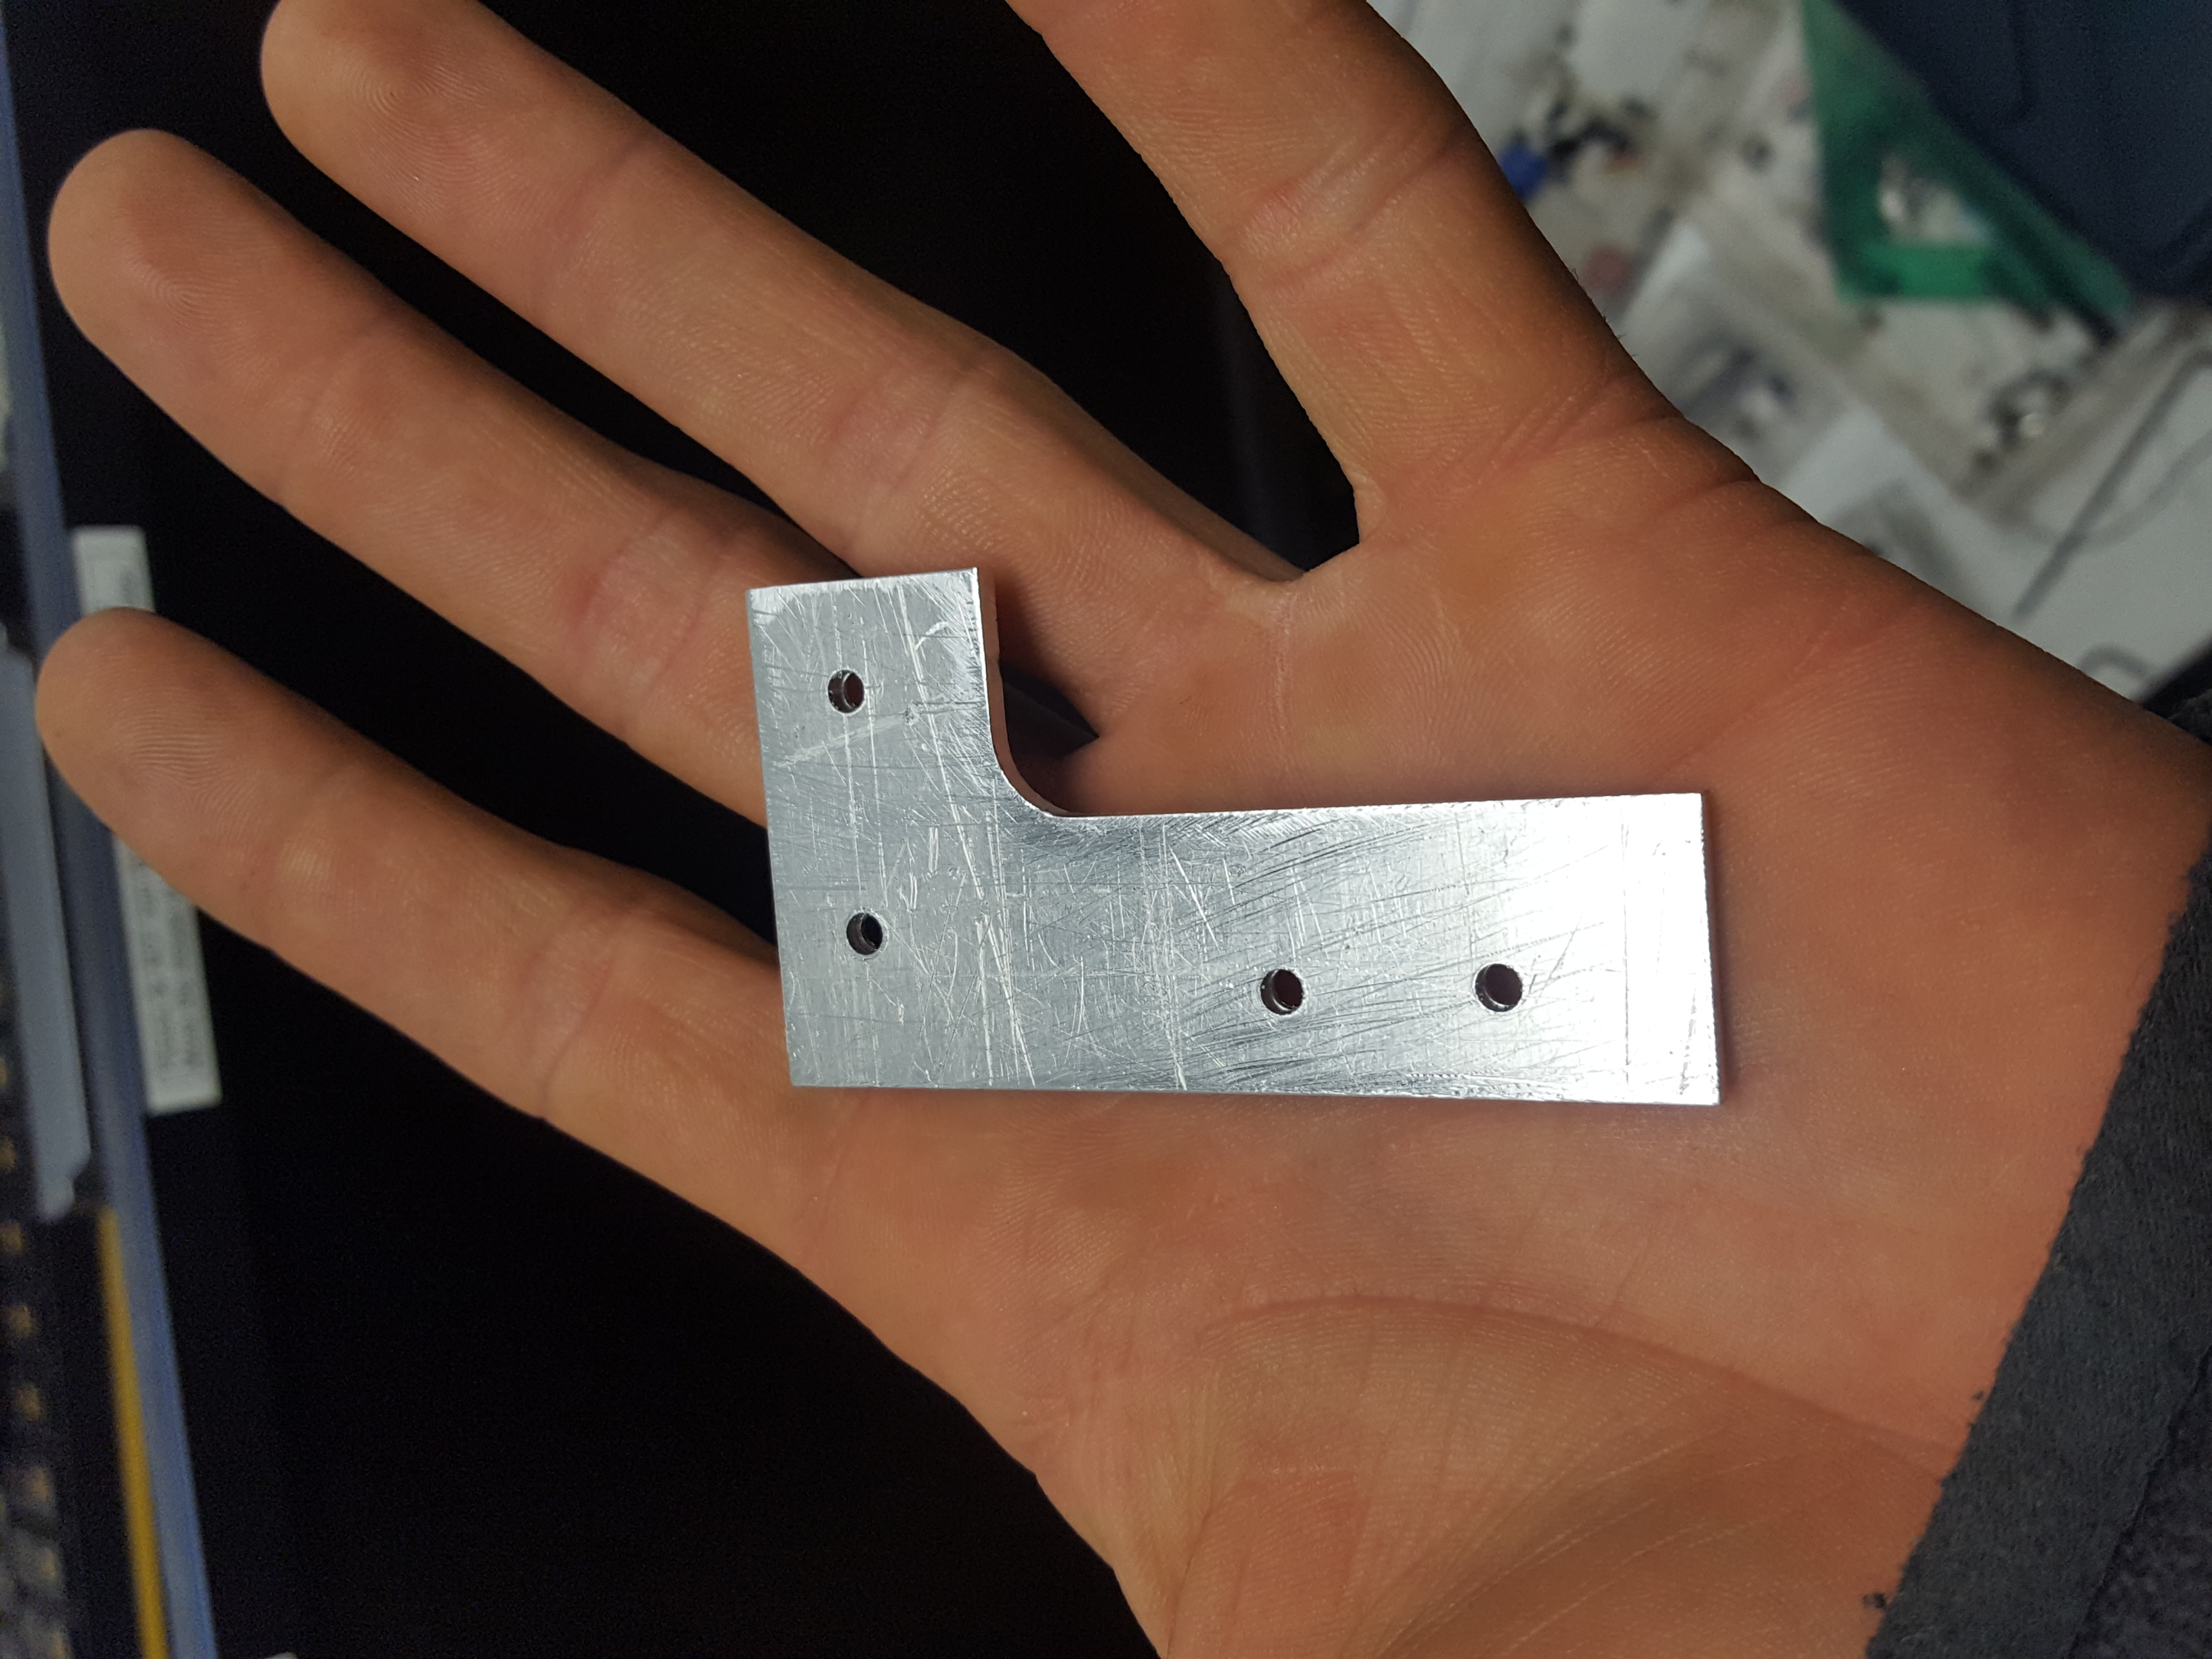
\includegraphics[scale=.025,angle=-90,origin=c]{images/bracket.jpg}
{\tiny Image: T.Hill}

				

			\end{frame}

		% section I subsection II
		\subsection{\sectionIsubsectionIItitle}\label{sectionIsubsectionII}

			\begin{frame}
				\frametitle{\sectionIsubsectionIItitle}
When a measurement system is {\PN \ublank}, its indicated value is compared directly with a {\BR \ublank}. This {\BR  \ublank \ublank} forms the basis of the comparison and is known as the {\OR \ublank}. This
{\OR \ublank} may be based on the output from a piece of equipment, from an object having a well-
defined physical attribute to be used as a comparison, or from a well-accepted technique known to
produce a reliable value.\vspace{5mm}\\

{\tiny Text: \underline{Theory and Design of Mechanical Measurements, 5th Edition}}
			
				
			\end{frame}


			\begin{frame}
				\frametitle{\sectionIsubsectionIItitle}
A {\GR \ublank} defines a physical variable that is used to describe some aspect of a physical system. A
{\PN \ublank} defines a quantitative measure of a dimension.\vspace{15mm}\\

{\tiny Text: \underline{Theory and Design of Mechanical Measurements, 5th Edition}}
			\end{frame}


		% section I subsection III
		\subsection{\sectionIsubsectionIIItitle}\label{sectionIsubsectionIII}
			\begin{frame} 
				\frametitle{\sectionIsubsectionIIItitle}
				\bigskip

				The dimension of mass is defined by the kilogram. Originally, the unit of the kilogram was defined
by the mass of one liter of water at room temperature. But today an equivalent yet more consistent
definition defines the kilogram exactly as the mass of a particular platinum-iridium cylindrical bar
that is maintained under very specific conditions at the International Bureau of Weights and
Measures located in Sevres, France. This particular bar (consisting of 90\% platinum and 10\%
iridium by mass) forms the primary standard for the kilogram. It remains today as the only basic unit
still defined in terms of a material object.

{\tiny Text: \underline{Theory and Design of Mechanical Measurements, 5th Edition}}


			\end{frame}	

			\begin{frame}[containsverbatim] 
				\frametitle{\sectionIsubsectionIIItitle}

				The {\BL \ublank \ublank} relate directly to a standard (historically).\vspc

\renewcommand{\arraystretch}{1.2}
\tagpdfsetup{table/header-rows={1}}
\begin{tabular}{|c|cc|cc|} \hline
\textbf{Unit}&\textbf{SI}&&\textbf{I-P}&\\ \hline\hline
Length&meter&$(m)$&foot&$(ft)$\\ \hline
Mass&kilogram&$(kg)$&slug&$(slug)$ \\\hline
Time&second&$(s)$&second&$(sec)$\\ \hline
Temperature&degrees&$(^\circ C$, $^\circ K)$&degrees&$(^\circ F$, $^\circ R)$ \\ \hline
Current&ampere&$(A)$&ampere&$(A)$\\ \hline
Substance&mole&$(mol)$&mole&$(mol)$\\ \hline
Light Intensity&candela&$(cd)$&candela&$(cd)$\\ \hline
%force&newton&(N)&pound&(lb)\\ \hline
%energy&joule&(J)&foot-pound&(ft-lb)\\ \hline
%power&watt&(W)&?&(ft-lb/sec)\\ \hline
\end{tabular}

				
			\end{frame}	

			\begin{frame} 
				\frametitle{\sectionIsubsectionIIItitle}
				\bigskip

				Common {\PN \ublank \ublank} are defined in terms of the the base units. \vspc
\renewcommand{\arraystretch}{1.2}
\tagpdfsetup{table/header-rows={1}}
\begin{tabular}{|c|cc|cc|} \hline
\textbf{Unit}&\textbf{SI} &&\textbf{I-P}&\\ \hline\hline
Force&newton&$(N)$&pound-force&$(lb_f)$\\ \hline
Voltage&volt&$(V)$&volt&$(V)$\\ \hline
Resistance&ohm&$(\Omega)$&ohm&$(\Omega)$\\ \hline
Capacitance&farah&$(F)$&farah&$(F)$ \\ \hline 
Inductance&henry&(H)&henry&(H)\\ \hline
Energy&joule&$(J)$&foot-pound&$(ft-lb)$\\ \hline
Power&watt&$(W)$&foot-pound per second&$(ft-lb/sec)$\\ \hline

\end{tabular}
			


			\end{frame}


		% section I subsection IV
		\subsection{\sectionIsubsectionIVtitle}\label{sectionIsubsectionIV}	

			\begin{frame} \scriptsize
				\frametitle{\sectionIsubsectionIVtitle}

				\bigskip

				The known value applied to a measurement system during calibration becomes the standard on which the calibration is based. \vspc 
So how do we pick this standard, and how good is it? \vspc
... primary standards are impractical as standards for normal calibration use ... there exists a hierarchy of reference and secondary standards used to duplicate the primary standards. \vspc
\tagpdfsetup{table/header-rows={1}}
\begin{tabular}{|lcl|}\hline\hline
{\OR \ublank} standard&---&Maintained as \ublank unit standard\\ \hline
{\PN \ublank} standard&---&Used to calibrate \ublank standards\\ \hline
{\PR \ublank} standard&---&Used to calibrate \ublank standards\\ \hline
{\BL \ublank} standard&---&Used to calibrate \ublank instruments\\ \hline 
\end{tabular}

\vspace{2mm}
{\tiny Text: \underline{Theory and Design of Mechanical Measurements, 5th Edition}}


				
			\end{frame}

			\begin{frame}
				\frametitle{\sectionIsubsectionIVtitle}

\bigskip
Examples of standards or using a standard:
\begin{itemize}
  \item -
  \item -
  \item -
\end{itemize}



			\end{frame}

	
	% Section II
	\section{\sectionIItitle}\label{sectionII}

		% section II Outline
		\begin{frame}
			\large \textbf{Topic 2 - \sectionIItitle} \vspace{3mm}\\

			\begin{itemize}
				\item \hyperref[sectionIIsubsectionI]{\sectionIIsubsectionItitle} \vspc %  section II subsection I
				\item \hyperref[sectionIIsubsectionII]{\sectionIIsubsectionIItitle} \vspc % section II subsection II
				\item \hyperref[sectionIIsubsectionIII]{\sectionIIsubsectionIIItitle} \vspc % section II subsection III
				\item \hyperref[sectionIIsubsectionIV]{\sectionIIsubsectionIVtitle} \vspc % section II subsection IV
			\end{itemize}

		\end{frame}

		% section II subsection I
		\subsection{\sectionIIsubsectionItitle}\label{sectionIIsubsectionI}

			\begin{frame}
				\frametitle{\sectionIIsubsectionItitle}


A {\BL \ublank} applies a known {\PN \ublank \ublank} to a measurement system for the purpose of observing the
system {\PR \ublank \ublank}. It establishes the relationship between the input and output values. The known
value used for the {\BL \ublank} is called the {\OR \ublank}. \vspc

\begin{itemize}
\item A range of input values can be used to form a calibration curve.
\item The calibration curve describes the input-output relationship of
the measurement system.
\end{itemize}

\vspace{10mm}
{\tiny Text: \underline{Theory and Design of Mechanical Measurements, 5th Edition}, }


			\end{frame}


		% section II subsection II
		\subsection{\sectionIIsubsectionIItitle}\label{sectionIIsubsectionII}

			\begin{frame}


      \textbf{Static Calibration Curve}
			\begin{multicols}{2}

        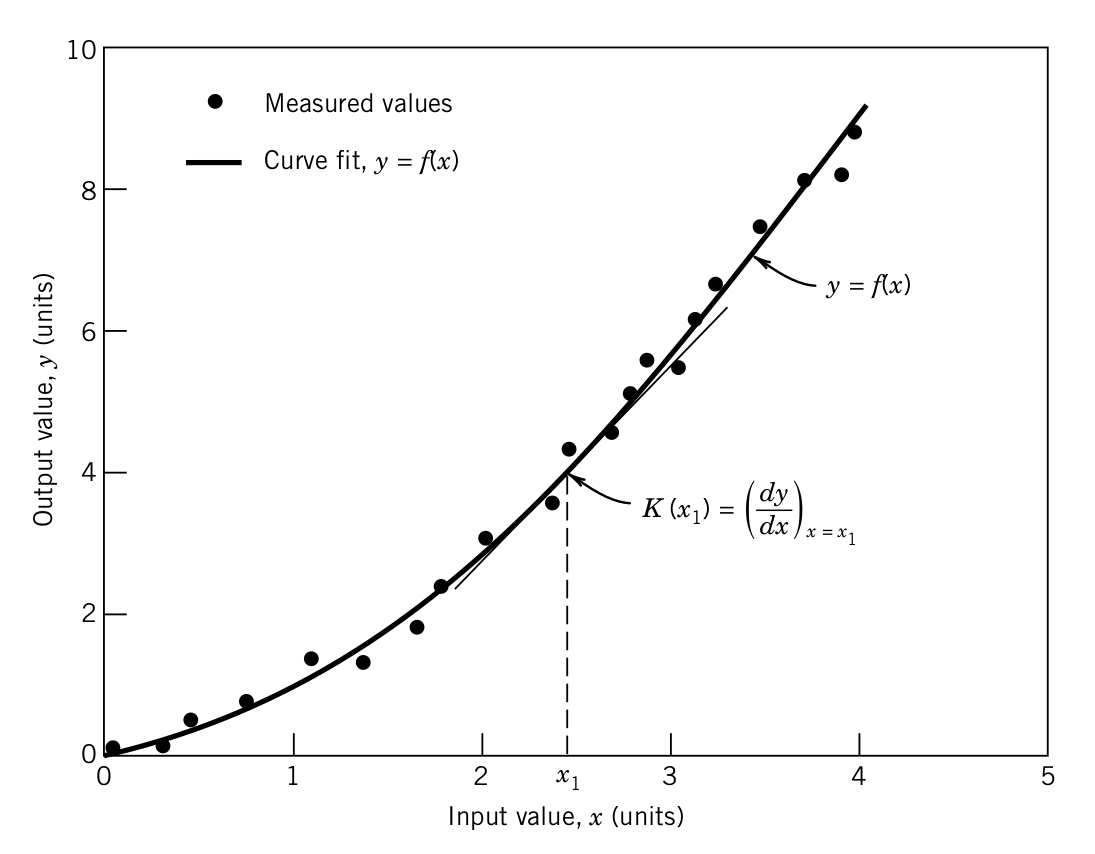
\includegraphics[scale=0.165]{images/calibration_curve.png}

        \hspace{20mm} {\bfseries y}: measured signal\vspc 
        \hspace{25mm} (output) \vspcc
        \hspace{20mm} {\bfseries x}: known standard\vspc
        \hspace{25mm} (input) \\
        \end{multicols}

        \textbf{Question:} How many values are needed for a calibration? Why?\vspc
        {\tiny Image: \underline{Theory and Design of Mechanical Measurements, 5th Edition}, }
          

			\end{frame}


		% section II subsection III
		\subsection{\sectionIIsubsectionIIItitle}\label{sectionIIsubsectionIII}

			\begin{frame}
				\frametitle{\sectionIIsubsectionIIItitle}

You have learned about these by a a different name. \vspcc

{\RD \ublank \ublank} - The Slope of the Calibration Curve \vspc

{\BL \ublank \ublank} - Y-Intercept of Calibration Curve \vspccc

\textbf{Question:} How many parameters or variables are needed to describe the curve?
			
			\end{frame}		

			\begin{frame}
				\frametitle{\sectionIIsubsectionIIItitle}

				\bigskip


				


			\end{frame}


		% section II subsection IV 
		\subsection{\sectionIIsubsectionIVtitle}\label{sectionIIsubsectionIV}

			\begin{frame}
				\frametitle{\sectionIIsubsectionIVtitle}

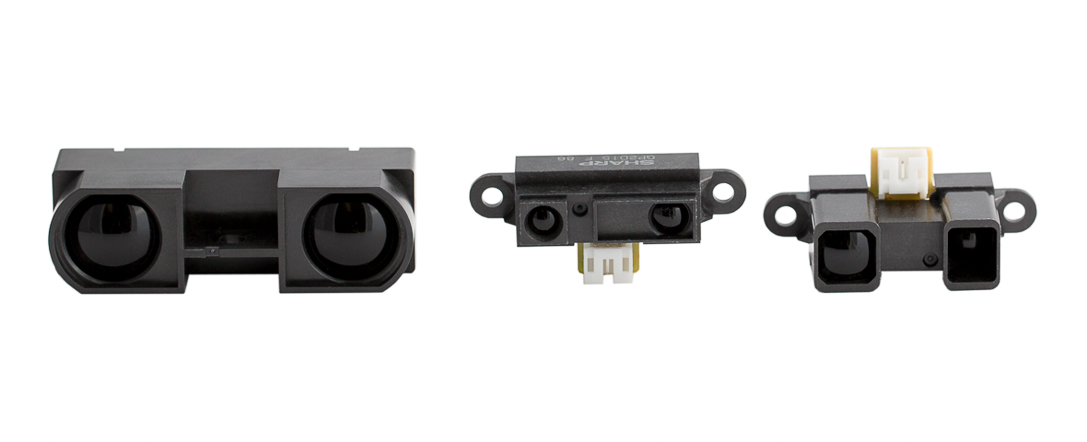
\includegraphics[scale=0.165]{images/sharp_ranger.jpg}

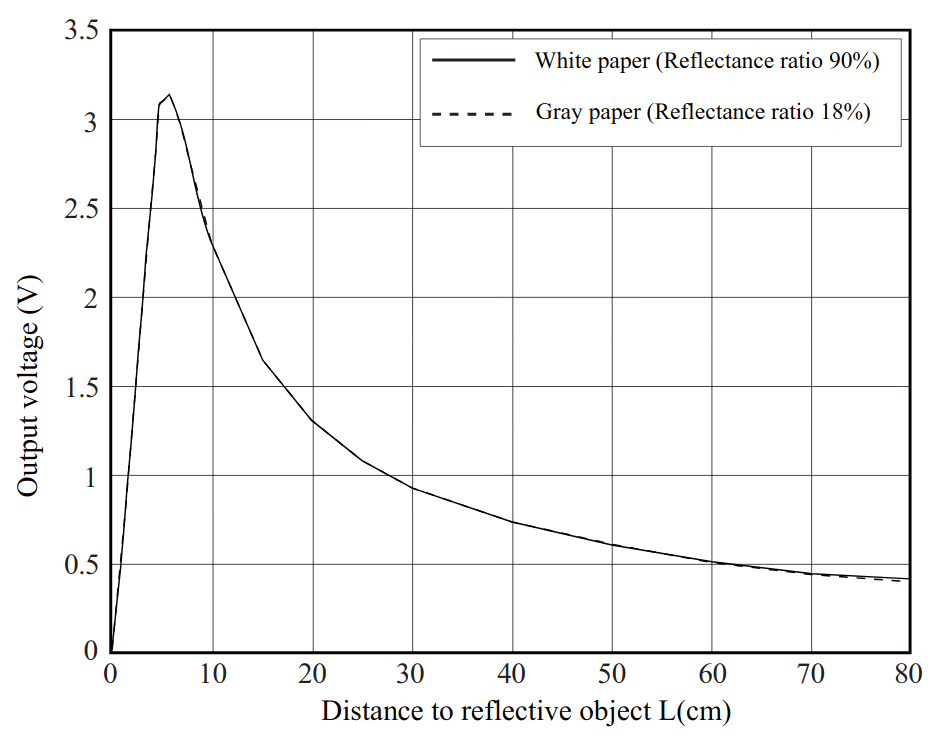
\includegraphics[scale=0.15]{images/sharp_calibration_fig1.png}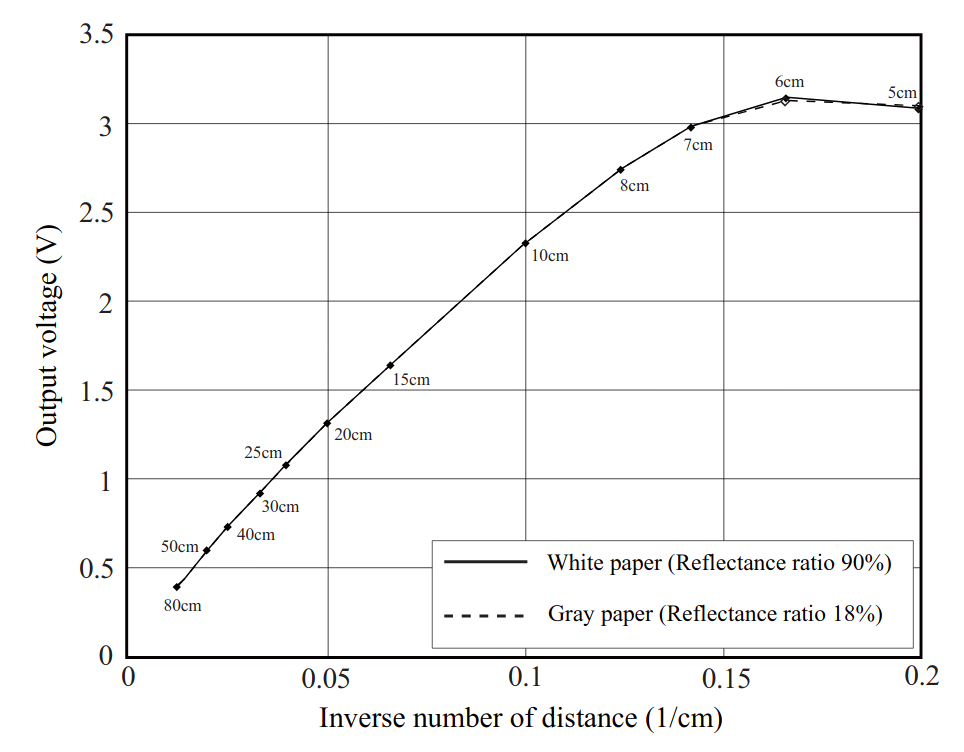
\includegraphics[scale=0.15]{images/sharp_calibration_fig2.png}

			\end{frame}

		
	% Section III
	\section{\sectionIIItitle}\label{sectionIII}

		% section III Outline
		\begin{frame}
			\large \textbf{Topic 3 - \sectionIIItitle} \vspace{3mm}\\

			\begin{itemize}
				\item \hyperref[sectionIIIsubsectionI]{\sectionIIIsubsectionItitle} \vspc %  section III subsection I
				\item \hyperref[sectionIIIsubsectionII]{\sectionIIIsubsectionIItitle} \vspc % section III subsection II
				\item \hyperref[sectionIIIsubsectionIII]{\sectionIIIsubsectionIIItitle} \vspc % section III subsection III
				\item \hyperref[sectionIIIsubsectionIV]{\sectionIIIsubsectionIVtitle} \vspc % section III subsection IV
				\item \hyperref[sectionIIIsubsectionV]{\sectionIIIsubsectionVtitle} \vspc % section III subsection V
			\end{itemize}

		\end{frame}

		% section III subsection I
		\subsection{\sectionIIIsubsectionItitle}\label{sectionIIIsubsectionI}

			\begin{frame}
				\frametitle{\sectionIIIsubsectionItitle}


A measured variable is often a function of one or more independent variables that are controlled during the measurement. ... This is a common procedure used to document the relationship between the measured variable and an independent process variable. ... \vspccc

We can use {\GR \ublank} analysis to establish a {\BL \ublank \ublank} between the {\PN \ublank} variable and the {\PR \ublank} variable. This discussion pertains directly to polynomial curve fits.\vspcc

Other functions such as exponential and log fits can also be used.

\vspace{10mm}
{\tiny Text: T.HIll, \underline{Theory and Design of Mechanical Measurements, 5th Edition} }

				
			\end{frame}

			\begin{frame}
				\frametitle{\sectionIIIsubsectionItitle}


       Consider the graphs below. This is a calibration curve.
 		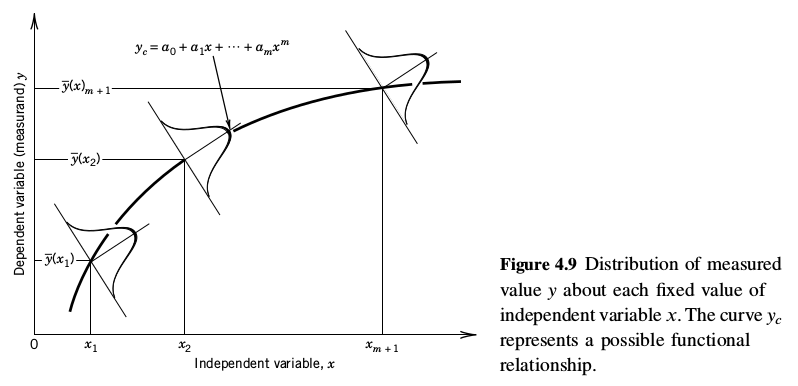
\includegraphics[scale=0.40]{images/lecture4_fig1.png}
 		{\tiny Image: \underline{Theory and Design of Mechanical Measurements, 5th Edition} }


		
			\end{frame}

		% section III subsection II
		\subsection{\sectionIIIsubsectionIItitle}\label{sectionIIIsubsectionII}	

			\begin{frame}
				\frametitle{\sectionIIIsubsectionIItitle}

	\begin{itemize}
		
		\item We are trying to find a polynomial of best fit for the data. \vspc
		\scalebox{1.0}{$y_c(x)=a_0+a_1x+a_2x^2+\dots+a_mx^m\hspace{10mm}m\leq(n-1)$} \vspc

		\item This is done by minimizing the quantity below.\vspc
		\scalebox{1.0}{$D=\Sigma_{i=1}^N(y_i-y_{ci})^2=\Sigma_{i=1}^N(y_i-a_0+a_1x+a_2x^2+\dots+a_mx^m)^2$} \vspc

		\item For a first order curve the coefficients become: \vspcc
		
		\scalebox{1.0}{$a_0=\frac{\Sigma x_i\Sigma x_i y_i-\Sigma x_i^2\Sigma y_i}{(\Sigma x_i)^2-N\Sigma x_i^2}$} \hspc, \scalebox{1.0}{$a_1=\frac{\Sigma x_i\Sigma y_i-N\Sigma x_i y_i }{(\Sigma x_i)^2-N\Sigma x_i^2}$}

	\end{itemize}

	

			\end{frame}

		% section III subsection III
		\subsection{\sectionIIIsubsectionIItitle}\label{sectionIIIsubsectionIII}

			\begin{frame}
				\frametitle{\sectionIIIsubsectionIIItitle}

		 Most spreadsheet and engineering software packages can perform a {\GR regression analysis} on a
data set. Examples will be shown throughout the course in MATLAB and EXCEL.\vspcc
	\begin{itemize}
	
	\item MATLAB - curve fitting toolbox - {\itshape polyfit()}
	\item Excel - {\itshape linest()}
	\item Python - {\itshape numpy.linalg.lstsq() }
	\item Labview - {\itshape Linear Fit VI, Exponential Fit VI, etc.}
	\item and many more...
	
	\end{itemize}
		

			\end{frame}

	
% section III subsection IV
		\subsection{\sectionIIIsubsectionIVtitle}\label{sectionIIIsubsectionIV}	

			\begin{frame}
				\frametitle{\sectionIIIsubsectionIVtitle}

\frametitle{Sample Calibration Data}
\tagpdfsetup{table/header-rows={1}}
\begin{tabular}{|c|c|c|}\hline
Sample \# & Known Distance $x_i (m)$ & Measured Voltage $y_i (V)$ \\ \hline \hline
1&6	&1.67 \\ \hline
2&9	&1.17 \\ \hline
3&12&0.89 \\ \hline
4&15&0.72 \\ \hline
5&18&0.61 \\ \hline
6&21&0.53 \\ \hline
\end{tabular}

\vspace{5mm}
Linear Least Squares Regression Coefficients: 
\scalebox{1}{$a_0= \hspc,\hspc a_1=$} \vspc

Functional Relationship: \\
\scalebox{1}{$y=a_1*x+a_0$}

			\end{frame}

			\begin{frame*}
				\frametitle{\sectionIIIsubsectionIVtitle}
				\frametitle{ Linear Regression in MATLAB - Manual}

%\begin{lrbox}{\mybox}

\begin{verbatim}

clear variables;close all;clc

x=[];
y=[];
n=length(x);

% perform Linear Least Squares Regression 
a0=
a1=

x_f=5.0:1.0:25;
y_f=

% generate 1st order curve fit with polyfit()
P1=polyfit(x,y,1);

x_f1=5.0:1.0:25;
y_f1=

\end{verbatim}

%\end{lrbox}

\scalebox{0.8}{\usebox{\mybox}}

\end{frame*}


			\begin{frame*}
				\frametitle{\sectionIIIsubsectionIVtitle}
			\frametitle{ Linear Regression in MATLAB - Manual}

%\begin{lrbox}{\mybox}

\begin{verbatim}
figure(1);hold on

plot(x,y,'r*')
plot(x_f,y_f,'m-')
plot(x_f1,y_f1,'b--')

title('First Order Calibration')
xlabel('Known Distance (m)')
ylabel('Measured Voltage (V)')
legend('Raw Data','Linear Fit (T.Hill)','Linear Fit (polyfit)')
grid on
\end{verbatim}

%\end{lrbox}

\scalebox{0.8}{\usebox{\mybox}}	


			\end{frame*}


			\begin{frame}
				\frametitle{\sectionIIIsubsectionIVtitle}
				\frametitle{ First Order Calibration Curve}

		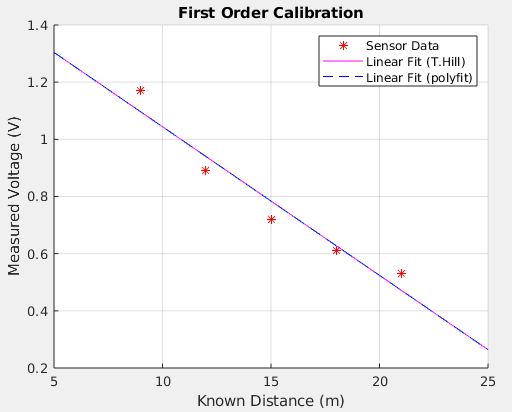
\includegraphics[scale=0.4]{images/calibration_fig2.png} 
 		{\tiny Images: T.Hill }


			\end{frame}

			\begin{frame}
				\frametitle{\sectionIIIsubsectionIVtitle}
				
\frametitle{ Fourth Order Calibration Curve}
		
		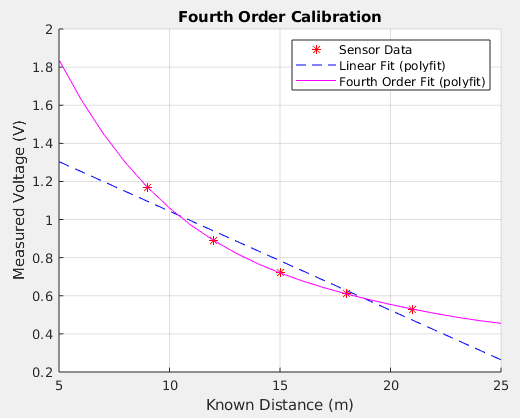
\includegraphics[scale=0.29]{images/calibration_fig1.png} \hspc  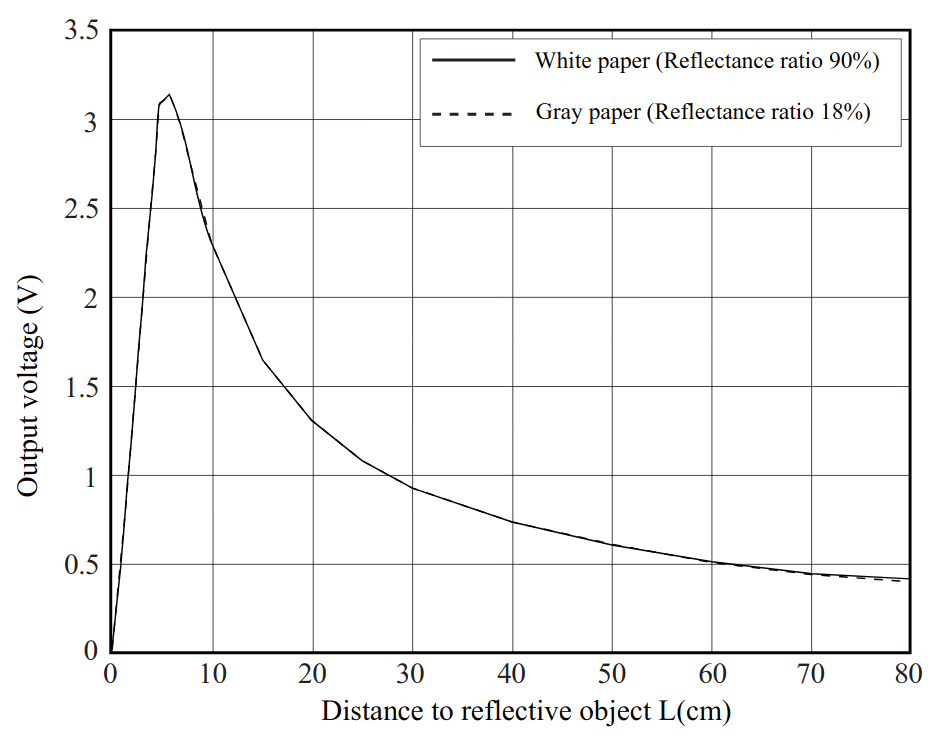
\includegraphics[scale=0.15]{images/sharp_calibration_fig1.png}\vspc
 		{\tiny Images: T.Hill, Sharp }

			\end{frame}



				% section III subsection V
		\subsection{\sectionIIIsubsectionVtitle}\label{sectionIIIsubsectionV}	

			\begin{frame}
				\frametitle{\sectionIIIsubsectionVtitle}

				\frametitle{ Activity: Sensor Calibration - IR Ranger} 

	\textbf{Groups of up to 2} - At least one computer is required.


	\textbf{Instructions:}
	\begin{enumerate} \scriptsize
		\item Use the sample calibration data provided to calculate the {\bfseries static sensitivity} and {\bfseries zero offset} of a 1st order regression line using a MATLAB program.  
		\item Show the calibration data and calibration curve on the same graph. Label the graph and show a legend.
		\item Show how the calibration curve could be used for a measurement application. Show two(2) example data points. 
		\item Modify your program to calculate an improved calibration curve using a different mathematical model. Discuss the qualities of each curve. Are there benifits and tradeoffs?
	\end{enumerate}


	\textbf{Submission:}
	\begin{itemize}\scriptsize
		\item Your code should calculate the required values and generate the required graphs. 
		\item Submit your MATLAB code to the appropriate ilearn folder. Include all names on the code. 
		\item Each group member must submit the complete assignment to recieve credit. 
	\end{itemize}


				\end{frame}

\end{document}





